\begin{figure}
  \centering

  \small

  \newcommand{\w}[1]{\textcolor{white}{#1}}
  \def\svgwidth{0.9\textwidth}

  % INKSCAPE
%% Creator: Inkscape inkscape 0.91, www.inkscape.org
%% PDF/EPS/PS + LaTeX output extension by Johan Engelen, 2010
%% Accompanies image file 'vape.eps' (pdf, eps, ps)
%%
%% To include the image in your LaTeX document, write
%%   \input{<filename>.pdf_tex}
%%  instead of
%%   \includegraphics{<filename>.pdf}
%% To scale the image, write
%%   \def\svgwidth{<desired width>}
%%   \input{<filename>.pdf_tex}
%%  instead of
%%   \includegraphics[width=<desired width>]{<filename>.pdf}
%%
%% Images with a different path to the parent latex file can
%% be accessed with the `import' package (which may need to be
%% installed) using
%%   \usepackage{import}
%% in the preamble, and then including the image with
%%   \import{<path to file>}{<filename>.pdf_tex}
%% Alternatively, one can specify
%%   \graphicspath{{<path to file>/}}
%% 
%% For more information, please see info/svg-inkscape on CTAN:
%%   http://tug.ctan.org/tex-archive/info/svg-inkscape
%%
\begingroup%
  \makeatletter%
  \providecommand\color[2][]{%
    \errmessage{(Inkscape) Color is used for the text in Inkscape, but the package 'color.sty' is not loaded}%
    \renewcommand\color[2][]{}%
  }%
  \providecommand\transparent[1]{%
    \errmessage{(Inkscape) Transparency is used (non-zero) for the text in Inkscape, but the package 'transparent.sty' is not loaded}%
    \renewcommand\transparent[1]{}%
  }%
  \providecommand\rotatebox[2]{#2}%
  \ifx\svgwidth\undefined%
    \setlength{\unitlength}{859.20961914bp}%
    \ifx\svgscale\undefined%
      \relax%
    \else%
      \setlength{\unitlength}{\unitlength * \real{\svgscale}}%
    \fi%
  \else%
    \setlength{\unitlength}{\svgwidth}%
  \fi%
  \global\let\svgwidth\undefined%
  \global\let\svgscale\undefined%
  \makeatother%
  \begin{picture}(1,0.69284606)%
    \put(0,0){\includegraphics[width=\unitlength]{vape.eps}}%
    \put(0.19164384,0.32189606){\color[rgb]{1,1,1}\makebox(0,0)[b]{\smash{}}}%
    \put(0.11429625,0.27347947){\color[rgb]{0,0,0}\makebox(0,0)[b]{\smash{$\mu_i$}}}%
    \put(0.11383134,0.58844779){\color[rgb]{0,0,0}\makebox(0,0)[b]{\smash{\w{$\pi_i$}}}}%
    \put(0.09389221,0.07975793){\color[rgb]{0,0,0}\makebox(0,0)[b]{\smash{}}}%
    \put(0.22819153,0.37577802){\color[rgb]{1,1,1}\makebox(0,0)[b]{\smash{\w{$\delta_i$}}}}%
    \put(0.23060784,0.03811878){\color[rgb]{0,0,0}\makebox(0,0)[b]{\smash{$\hat{\mu}_i$}}}%
    \put(0.23010837,0.58769977){\color[rgb]{0,0,0}\makebox(0,0)[b]{\smash{\w{$\hat{\pi}_i$}}}}%
    \put(0.22810895,0.27444915){\color[rgb]{1,1,1}\makebox(0,0)[b]{\smash{\w{$\varepsilon_i$}}}}%
    \put(0.17856811,0.66454141){\color[rgb]{0,0,0}\makebox(0,0)[b]{\smash{\footnotesize \w{$p_{i}^1$}}}}%
    \put(0.17872829,0.52176623){\color[rgb]{0,0,0}\makebox(0,0)[b]{\smash{\tiny \w{$1$}}}}%
    \put(0.61317851,0.04185319){\color[rgb]{0,0.78431373,1}\makebox(0,0)[b]{\smash{\footnotesize $\alpha_{i,i+1}$}}}%
    \put(0.52289597,0.48249583){\color[rgb]{0,0.48235294,0.61568627}\makebox(0,0)[lb]{\smash{\footnotesize $\alpha_{i,i+1}^2$}}}%
    \put(0.52187714,0.61541525){\color[rgb]{0.62352941,0,0.52941176}\makebox(0,0)[lb]{\smash{\footnotesize $\alpha_{i,i+1}^2$}}}%
    \put(0.36026177,0.03814947){\color[rgb]{0,0,0}\makebox(0,0)[b]{\smash{$1$}}}%
    \put(0.31020706,0.52364148){\color[rgb]{0,0,0}\makebox(0,0)[b]{\smash{\tiny \w{$\nu_i$}}}}%
    \put(0.01170748,0.65362397){\color[rgb]{0,0,0}\makebox(0,0)[lb]{\smash{1}}}%
    \put(0.01137256,0.55389274){\color[rgb]{0,0,0}\makebox(0,0)[lb]{\smash{2}}}%
    \put(0.00640934,0.47847459){\color[rgb]{0,0,0}\makebox(0,0)[lb]{\smash{3\textsf{A}}}}%
    \put(0.00640974,0.32391393){\color[rgb]{0,0,0}\makebox(0,0)[lb]{\smash{3\textsf{B}}}}%
    \put(0.01114481,0.18425069){\color[rgb]{0,0,0}\makebox(0,0)[lb]{\smash{4}}}%
    \put(0.0063866,0.13210975){\color[rgb]{0,0,0}\makebox(0,0)[lb]{\smash{5\textsf{A}}}}%
    \put(0.0063866,0.07717554){\color[rgb]{0,0,0}\makebox(0,0)[lb]{\smash{5\textsf{B}}}}%
    \put(0.01146873,0.02689677){\color[rgb]{0,0,0}\makebox(0,0)[lb]{\smash{6}}}%
    \put(0.31404356,0.13445759){\color[rgb]{1,0,0.84705882}\makebox(0,0)[lb]{\smash{\tiny $\exp(\omega_i)$}}}%
    \put(0.82243657,0.27319795){\color[rgb]{0,0,0}\makebox(0,0)[b]{\smash{$\mu_{i+1}$}}}%
    \put(0.82010953,0.58816626){\color[rgb]{0,0,0}\makebox(0,0)[b]{\smash{\w{$\pi_{i+1}$}}}}%
    \put(0.93074537,0.3754965){\color[rgb]{1,1,1}\makebox(0,0)[b]{\smash{\w{$\delta_{i+1}$}}}}%
    \put(0.93688609,0.03783723){\color[rgb]{0,0,0}\makebox(0,0)[b]{\smash{$\hat{\mu}_{i+1}$}}}%
    \put(0.93266221,0.58741824){\color[rgb]{0,0,0}\makebox(0,0)[b]{\smash{\w{$\hat{\pi}_{i+1}$}}}}%
    \put(0.93066279,0.27416763){\color[rgb]{1,1,1}\makebox(0,0)[b]{\smash{\w{$\varepsilon_{i+1}$}}}}%
    \put(0.88314427,0.52148471){\color[rgb]{0,0,0}\makebox(0,0)[b]{\smash{\tiny \w{$1$}}}}%
    \put(0.82639142,0.0682316){\color[rgb]{0,0,0}\makebox(0,0)[b]{\smash{$\mu_{i+1}$}}}%
    \put(0.11825105,0.06851314){\color[rgb]{0,0,0}\makebox(0,0)[b]{\smash{$\mu_i$}}}%
  \end{picture}%
\endgroup%

  \caption{The coupling between a hierarchical level $i$ with its parent $i+1$ in the case of \textsf{VAPE} coupling, using within-trial dynamics: introducing $\nu$ as the (tonic) volatility estimation.}
  \label{\figlabel}
\end{figure}
